%Группа 9-2 Модуль 3
\cheadbf{Занятие 2}
\begin{listofex}
	\item Для объектов, указанных в таблице, определите, какими цифрами они обозначены на плане. Заполните таблицу, в ответ запишите последовательность четырех цифр.
	\begin{center}
		\footnotesize
		\begin{tabular}{|g|c|c|c|c|}
			\hline
			\textbf{Объекты}&Книжный шкаф&Диван&Торшер&Стул\\
			\hline
			\textbf{Цифры}&&&&\\
			\hline
		\end{tabular}
	\end{center}
	\begin{center}
		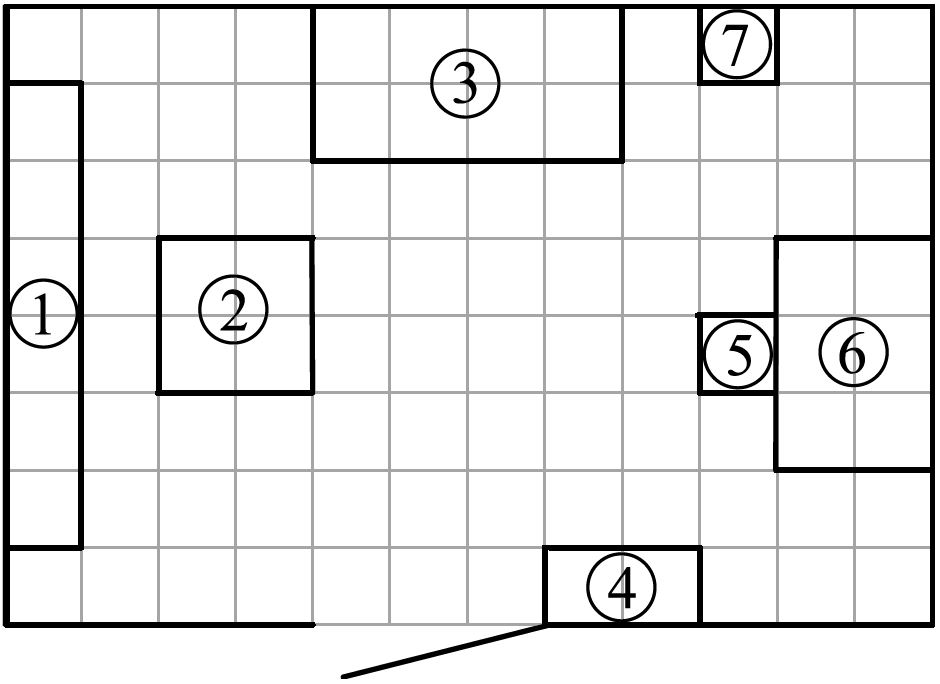
\includegraphics[align=t, width=0.3\textwidth]{pics/G91M3C2-1}
	\end{center}
	
	Владелец собирается провести ремонт своей квартиры. На плане изображена предполагаемая расстановка
	мебели в гостиной после ремонта. Сторона каждой клетки равна \( 0,4 \) м. Гостиная имеет прямоугольную
	форму. Единственная дверь гостиной деревянная, в стене напротив двери расположено окно. Справа от двери
	будет поставлен комод, слева от двери у стены будет собран книжный шкаф. В глубине комнаты у стены
	планируется поставить диван. Перед книжным шкафом будет поставлено кресло. Справа от дивана будет
	стоять торшер. Площадь, занятая диваном, по плану будет равна \( 1,28 \) м\( ^2 \). У стены справа от двери
	планируется поставить письменный стол, а перед ним поставить стул. Пол гостиной (в том числе там, где
	будет стоять мебель) планируется покрыть паркетной доской размером \( 40 \) см \( \times \) \( 20 \) см. Кроме того, владелец
	квартиры планирует смонтировать в гостиной электрический подогрев пола. Чтобы сэкономить, владелец не
	станет подводить обогрев под книжный шкаф, кресло, диван и комод, а также на участок площадью \( 0,16 \) м\( ^2 \)
	между диваном и торшером.
	\item Паркетная доска продаётся в упаковках по \( 15 \) штук. Сколько упаковок с паркетной доской нужно
	купить, чтобы покрыть пол гостиной?
	\item Найдите площадь той части гостиной, на которой будет смонтирован электрический подогрев пола. Ответ дайте в м\( ^2 \).
	\item Найдите расстояние d между противоположными углами кресла (диагональ). Ответ дайте в метрах в формате \( \dfrac{d}{\sqrt{2}} \).
	\item Владелец квартиры выбирает торшер из двух моделей \( A \) и \( B \). Цена торшеров и их среднее суточное потребление электроэнергии указаны в таблице. Цена электроэнергии составляет \( 4 \) рубля за кВт \( \cdot \) ч.
	\begin{center}
		\footnotesize
		\begin{tabular}{|c|c|x{8cm}|}
			\hline
			\rowcolor{gray}\textbf{Модель}&\textbf{Цена торшера (руб.)}&\textbf{Среднее потребление электроэнергии в сутки, кВт \( \cdot \) ч}\\
			\hline
			\( A \)&\( 2\:000 \)&\( 0,2 \)\\
			\hline
			\( B \)&\( 1\:200 \)&\( 0,3 \)\\
			\hline
		\end{tabular}
	\end{center}
	Обдумав оба варианта, владелец квартиры выбрал модель \( A \). Через сколько лет непрерывной работы экономия от меньшего расхода электроэнергии окупит разницу в цене этих торшеров? Ответ округлите до целого числа в большую сторону.
	\item Пользуясь описанием, определите, какими цифрами на плане обозначены населённые пункты. В ответ запишите последовательность трёх цифр без пробелов, запятых и других дополнительных символов.
	\begin{center}
		\footnotesize
		\begin{tabular}{|g|c|c|c|}
			\hline
			\textbf{Населенные пункты}&д. Камышевка&д. Ясная&д. Хомяково\\
			\hline
			\textbf{Цифры}&&&\\
			\hline
		\end{tabular}
	\end{center}
	
	Полина летом отдыхает у дедушки в деревне Ясная. В четверг они собираются съездить на велосипедах в
	село Майское в магазин. Из деревни Ясная в село Майское можно проехать по прямой лесной дорожке. Есть
	более длинный путь: по прямолинейному шоссе через деревню Камышёвка до деревни Хомяково, где нужно
	повернуть под прямым углом налево
	на другое шоссе, ведущее в село Майское. Есть и третий маршрут: в деревне Камышёвка можно свернуть на
	прямую тропинку в село Майское, которая идёт мимо пруда.
	Лесная дорожка и тропинка образуют с шоссе прямоугольные треугольники.
	\begin{center}
		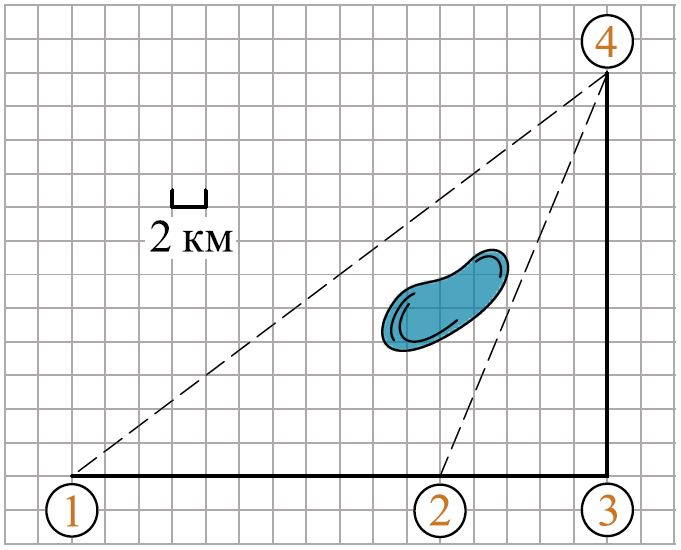
\includegraphics[align=t, width=0.3\textwidth]{pics/G91M3C2-2}
	\end{center}
	По шоссе Полина с дедушкой едут со скоростью 20 км/ч, а по лесной дорожке и тропинке --- со
	скоростью \( 15 \) км/ч. На плане изображено взаимное расположение населенных пунктов, длина стороны каждой клетки равна \( 2 \) км.
	\item Сколько километров проедут Полина с дедушкой от деревни Ясная до села Майское, если они поедут по шоссе через деревню Хомяково?
	\item Найдите расстояние от деревни Ясная до села Майское по прямой. Ответ дайте в километрах.
	\item Сколько минут затратят на дорогу из деревни Ясная в село Майское Полина с дедушкой, если поедут через деревню Хомяково?
	\item В таблице указана стоимость (в рублях) некоторых продуктов в четырех магазинах, расположенных в деревне Ясная, селе Майское, деревне Камышёвка и деревне Хомяково.
	\begin{center}
		\footnotesize
		\begin{tabular}{|c|c|c|c|c|}
			\hline
			\rowcolor{gray}\textbf{Продукт}&\textbf{д. Ясная}&\textbf{с. Майское}&\textbf{д. Камышевка}&\textbf{д. Хомяково}\\
			\hline
			Молоко (1 л)&42&38&41&33\\
			\hline
			Хлеб (1 батон)&25&21&29&30\\
			\hline
			Сыр Российский (1 кг)&310&320&290&280\\
			\hline
			Говядина (1 кг)&340&380&410&390\\
			\hline
			Картофель (1 кг)&15&20&17&18\\
			\hline
		\end{tabular}
	\end{center}
	Полина с дедушкой хотят купить \( 2 \) л молока, \( 3 \) кг говядины и \( 2 \) кг картофеля. В каком магазине такой набор продуктов будет стоить дешевле всего? В ответ запишите стоимость данного набора в этом магазине.
	\item \exercise{211}
	\item \exercise{445}
	\item \exercise{647}
	\item Найдите значение выражения \( \dfrac{16x-25y}{4\sqrt{x}-5\sqrt{y}}-\sqrt{y} \), если \( \sqrt{x}+\sqrt{y}=3 \)
	\item Найдите значение выражения \( \sqrt{(4\sqrt{2}-7)^2}+4\sqrt{2} \)
	\item Сократите дробь \( \dfrac{45^n}{3^{2n-1}\cdot5^{n-2}} \)
	\item Решите неравенство \( -x-2x\le0 \).\\ \selectanswer
	\begin{enumcols}[itemcolumns=2]
		\item \( (-\infty;-2)\cup[0;+\infty) \)
		\item \( (-\infty;-2]\cup(0;+\infty) \)
		\item \( (-2;0) \)
		\item \( [-2;0] \)
	\end{enumcols}
\end{listofex}
%\newpage
%\title{Домашняя работа №1}
%\begin{listofex}
%	
%\end{listofex}
%\newpage
%\title{Занятие №3}
%\begin{listofex}
%	
%\end{listofex}
%\newpage
%\title{Занятие №4}
%\begin{listofex}
%	
%\end{listofex}
%\newpage
%\title{Домашняя работа №2}
%\begin{listofex}
%	
%\end{listofex}
%\newpage
%\title{Занятие №5}
%\begin{listofex}
%	
%\end{listofex}
%\newpage
%\title{Занятие №6}
%\begin{listofex}
%	
%\end{listofex}
%\newpage
%\title{Домашняя работа №3}
%\begin{listofex}
%	
%\end{listofex}
%\newpage
%\title{Подготовка к проверочной работе}
%\begin{listofex}
%	
%\end{listofex}
%\newpage
%\title{Проверочная работа}
%\title{Вариант 1}
%\begin{listofex}
%	
%\end{listofex}
%\newpage
%\title{Проверочная работа}
%\begin{listofex}
%	
%\end{listofex}
\newpage
\chead{}
\begin{listofex}
	\item Решить уравнение:
	\begin{enumcols}[itemcolumns=2]
		\item \exercise{1034}
		\item \exercise{1033}
		\item \exercise{519}
	\end{enumcols}
	\item Решить систему уравнений:
	\begin{enumcols}[itemcolumns=2]
		\item \exercise{234}
		\item
		\( \left\{
		\begin{array}{l}
			x+y=6,\\
			x^2-y^2=12
		\end{array}
		\right. \)
		\item
		\( \left\{
		\begin{array}{l}
			x^3+y^3=7,\\
			x^2y+xy^2=-2
		\end{array}
		\right. \)
	\end{enumcols}
\end{listofex}